\documentclass[border=4pt,varwidth=17cm]{standalone}
\usepackage{amsmath,amssymb,mathrsfs,mathtools}
\usepackage{tikz}
\usetikzlibrary{positioning,fit,backgrounds,arrows.meta}
\def\RR{{\mathbb R}}\def\eps{\varepsilon}\def\then{\Rightarrow}
\def\J{\mathcal{J}_L}\def\A{\mathcal{A}_{f,g}}\def\Sol{\mathcal{S}_{f,g}}
\def\limsup{\mathop{\overline{\lim}}}\def\liminf{\mathop{\underline{\lim}}}
\def\Of{{\sf (O$_f$)}}\def\Og{{\sf (O$_g$)}}
\def\Rv{{\sf (R$_{\rm v}$)}}\def\Rh{{\sf (R$_{\rm h}$)}}
\begin{document}


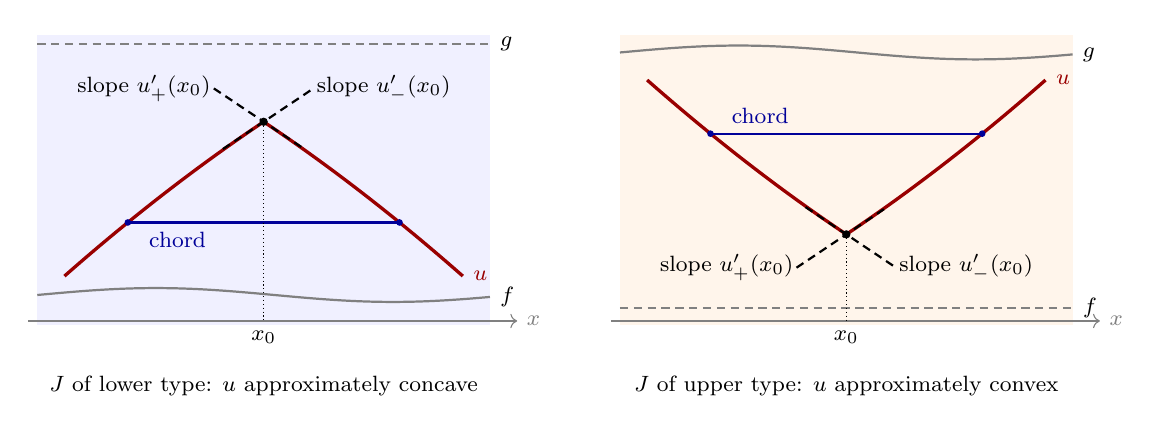
\begin{tikzpicture}[font=\footnotesize]
% left: lower type
\begin{scope}[x=1.15cm, y=1.1cm, declare function={U(\t)=2.3-0.7*abs(\t-2.5)-0.05*(\t-2.5)^2; F(\t)=0.3+0.08*sin(deg(1.2*\t));}]
  \fill[blue!6] (0,-0.05) rectangle (5,3.3);
  \draw[->, gray] (-0.1,0) -- (5.3,0) node[right] {$x$};
  \draw[thick, gray, domain=0:5, samples=60, smooth] plot (\x,{F(\x)}) node[right, black] {$f$};
  \draw[thick, gray, densely dashed] (0,3.2) -- (5,3.2) node[right, black] {$g$};
  \draw[very thick, red!60!black, domain=0.3:2.5, samples=40] plot (\x,{U(\x)});
  \draw[very thick, red!60!black, domain=2.5:4.7, samples=40] plot (\x,{U(\x)}) node[right] {$u$};
  % chord below u
  \draw[thick, blue!60!black] (1.0,{U(1.0)}) -- (4.0,{U(4.0)});
  \fill[blue!60!black] (1.0,{U(1.0)}) circle (1.2pt) (4.0,{U(4.0)}) circle (1.2pt);
  \node[blue!60!black, below] at (1.55,{U(1.0)}) {chord};
  % half tangents
  \draw[thick, densely dashed] (2.05,{2.3-0.7*0.45}) -- (3.05,{2.3+0.7*0.55});
  \draw[thick, densely dashed] (1.95,{2.3+0.7*0.55}) -- (2.95,{2.3-0.7*0.45});
  \fill (2.5,2.3) circle (1.5pt);
  \node[right, inner sep=1pt] at (3.05,{2.3+0.7*0.55}) {slope $u^\prime_-(x_0)$};
  \node[left, inner sep=1pt] at (1.95,{2.3+0.7*0.55}) {slope $u^\prime_+(x_0)$};
  \draw[densely dotted] (2.5,2.3) -- (2.5,0) node[below] {$x_0$};
  \node at (2.5,-0.75) {$J$ of lower type: $u$ approximately concave};
\end{scope}
% right: upper type
\begin{scope}[shift={(7.4,0)}, x=1.15cm, y=1.1cm, declare function={V(\t)=1.0+0.7*abs(\t-2.5)+0.05*(\t-2.5)^2; G(\t)=3.1+0.08*sin(deg(1.2*\t));}]
  \fill[orange!8] (0,-0.05) rectangle (5,3.3);
  \draw[->, gray] (-0.1,0) -- (5.3,0) node[right] {$x$};
  \draw[thick, gray, domain=0:5, samples=60, smooth] plot (\x,{G(\x)}) node[right, black] {$g$};
  \draw[thick, gray, densely dashed] (0,0.15) -- (5,0.15) node[right, black] {$f$};
  \draw[very thick, red!60!black, domain=0.3:2.5, samples=40] plot (\x,{V(\x)});
  \draw[very thick, red!60!black, domain=2.5:4.7, samples=40] plot (\x,{V(\x)}) node[right] {$u$};
  % chord above u
  \draw[thick, blue!60!black] (1.0,{V(1.0)}) -- (4.0,{V(4.0)});
  \fill[blue!60!black] (1.0,{V(1.0)}) circle (1.2pt) (4.0,{V(4.0)}) circle (1.2pt);
  \node[blue!60!black, above] at (1.55,{V(1.0)}) {chord};
  % half tangents
  \draw[thick, densely dashed] (2.05,{1.0+0.7*0.45}) -- (3.05,{1.0-0.7*0.55});
  \draw[thick, densely dashed] (1.95,{1.0-0.7*0.55}) -- (2.95,{1.0+0.7*0.45});
  \fill (2.5,1.0) circle (1.5pt);
  \node[right, inner sep=1pt] at (3.05,{1.0-0.7*0.55}) {slope $u^\prime_-(x_0)$};
  \node[left, inner sep=1pt] at (1.95,{1.0-0.7*0.55}) {slope $u^\prime_+(x_0)$};
  \draw[densely dotted] (2.5,1.0) -- (2.5,0) node[below] {$x_0$};
  \node at (2.5,-0.75) {$J$ of upper type: $u$ approximately convex};
\end{scope}
\end{tikzpicture}


\end{document}
